\chapter{Überblick über den praktischen Teil}\label{sec:experimente}
Im zweiten Teil dieser Arbeit werden die in Kapitel \ref{sec:wissenschaft} theoretisch betrachteten Methoden praktisch auf einer GPU ausgeführt und evaluiert. Der Überblick über das experimentelle Setup wird in Kapitel \ref{sec:setup} vorgestellt. In Kapitel \ref{sec:konzept} wird das Konzept des praktischen Teils der Arbeit erläutert.

\section{Experimentelles Setup}\label{sec:setup}
\subsection{Hardware}
Die Hardware umfasst einen Server mit 4 GPUs.
Von diesen 4 GPUs haben 2 GPUs jeweils den gleichen Typ:
\begin{itemize}
 \item Geforce GTX 1080 Ti
 \item Geforce RTX 2080 Ti 
\end{itemize}

Beide GPU-Typen arbeiten mit der CUDA Version 10.1. 

Während der Vorbereitung auf diese Experimente hat sich gezeigt, dass Experimente mit einer Geforce GTX 1080 Ti mit den Experimenten der Geforce RTX 2080 Ti nicht vergleichbar sind. Weiterhin lässt sich durch das Verwenden von gemischt präzisen Zahlen nur auf der Geforce RTX 2080 ein Geschwindigkeitsvorteil beim Training feststellen. Aus diesen zwei Gründen wurden alle Experimente auf der Geforce RTX 2080 Ti ausgeführt.  


\subsection{Wahl des Frameworks}

Es wird mit pytorch gearbeitet, da pytorch gegenüber anderen Frameworks eine grössere Flexibiltät erlaubt. Ausserdem ist eine fast vollständige Implementierung von PruneTrain in Pytorch geschrieben. Diese wird im nächsten Kapitel untersucht und soweit erweitert, dass es dem Stand im PruneTrain Paper entspricht.

Pytorch bietet mit cudnn und cuda im Hintergrund gute Möglichkeiten die Trainingszeiten einzelner Epochen zu messen und sie so mit einander zu vergleichen.


\subsection{verwendete Netzarchitektur}\label{sec:archi}
Die PruneTrain Implementierung hat initial mehrere verschiedene Netzarchitekturen zur Auswahl:
\begin{itemize}
 \item AlexNet
 \item ResNet 32/50
 \item vgg 8/11/13/16
 \item mobilenet
\end{itemize}

Diese Auswahl an Netzarchitekturen ist zu umfangreich, um alle diese Architekturen auf den vorgestellten Methoden zu evaluieren. Daher wird im Rahmen dieser Arbeit nur auf ResNet gearbeitet. Diese Entscheidung liegt daran, dass Resnets durch ihre Kurzschlussverbindungen gut mit sehr tiefen Netzstrukturen unmgehen können, ohne grosses Klassifikationsleistungsverluste dank Overfitting. Dies ist vorallem wichtig, wenn das Netz mit Hilfe des Operator für tieferes Netz noch tiefer gemacht werden soll. Die ResNet Struktur wird in der Implementierung so verändert, dass angeben werden kann wie tief das Netz sein soll. Das ResNet wird hier nicht mehr nur mit einer Zahl identifiziert sondern es wird angegeben, wieviele
\begin{itemize}
 \item $s$: Anzahl an Phasen, die das ResNet hat
 \item $N=[n_1, \ldots, n_S]:$ Anzahl von Blöcken pro Phase 
 \item $l$: Anzahl von (Conv+Batch)-Layer pro Block
 \item $[k_1, \ldots,k_S ]:$ Breite der Schichten je Phase
 \item $b$: Boolean Parameter, der angibt ob die Blöcke im Netz die Bootleneck-Eigenschaft haben
\end{itemize}
das jeweilige ResNet hat. Diese Vorgehensweise hat den Vortei, dass für ein im Verlauf tieferes beziehungweise breitere Netz eine Vergleichsmöglichkeit besteht. Dies bedeutet, dass das Netz welches im Verlauf entsteht auch direkt erstellt werden kann.


\color{blue1}
\subsection{Baseline Netz}\label{sec:baseline}
Um die Ergebnisse der Experimente in den folgenden Kapiteln einschätzen zu können wird ein ResNet, ohne Anpassungen um Trainingszeit zu sparen, trainiert. In Tabelle \ref{tab:baseline} ist die Struktur dieses Netze zu sehen. Das breite Baseline-Netz wird dabei für die Evaluierung des Beschneiden des Netzes verwendet. Das schmallere Baseline-Netz wird für die Evaluierung der Methoden, die das Netz breiter machen verwendet.

Das Netz hat drei Phasen $(s=3)$, wobei jeder der Phasen 5 Blöcke hat $(N=[5,5,5])$. Pro Basisblock sind zwei (Conv+Batch)-Schichten vorhanden $(l=3)$. Bei einem Übergangsblock, der als erster Block in einer neuen Phase bei einer Vergrösserung der Bereit beim Phasenübergang genutzt wird ist eine (Conv+Schicht)-Schicht mehr vorhanden. Eine grafische Darstellung der Blöcke ist in Abbildung \ref{abb:blocks} zu sehen.




\begin{figure}[h]
   \begin{minipage}[b]{.4\linewidth} % [b] => Ausrichtung an \caption
      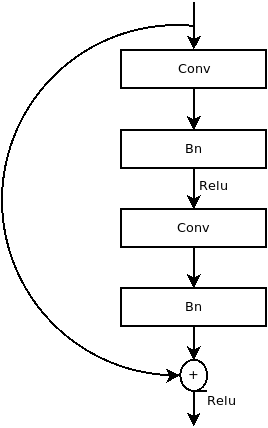
\includegraphics[width=0.8\linewidth]{KapitelPartB/Images/Basisblock.png}
      \caption{Basisblock}
   \end{minipage}
   \hspace{.1\linewidth}% Abstand zwischen Bilder
   \begin{minipage}[b]{.4\linewidth} % [b] => Ausrichtung an \caption
      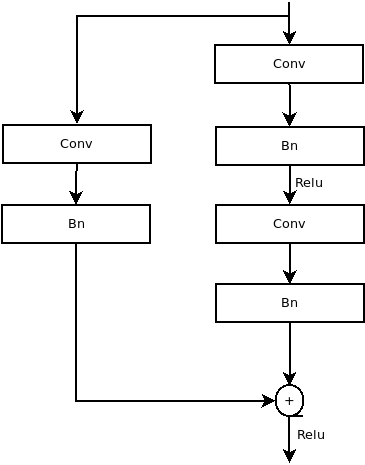
\includegraphics[width=0.8\linewidth]{KapitelPartB/Images/Ubergangsblock.png}
      \caption{Übergangsblock}
   \end{minipage}
   \caption{Grafische Darstellung Basis- und Übergangsblock}
   \label{abb:blocks}
\end{figure}

\begin{table}[H]
\begin{tabular}{|l|l|l|l|l|l|}
\hline
      &                & \multicolumn{2}{c|}{breites Baseline-Netz} &\multicolumn{2}{c|}{schmalles Baseline-Netz} \\ 
Phase & Schicht/Block  & \#Eingangs- & \#Ausgangs-       & \#Eingangs- & \#Ausgangs-    \\
      &                & \multicolumn{2}{c|}{kanäle}     & \multicolumn{2}{c|}{kanäle}  \\ \hline
      & Conv 1 + Bn 1  & 3                & 16           & 3           & 8              \\ \hline \hline
1     & Basisblock     & 16               & 16           & 8           & 8              \\ \hline
      & Basisblock     & 16               & 16           & 8           & 8              \\ \hline
      & Basisblock     & 16               & 16           & 8           & 8              \\ \hline
      & Basisblock     & 16               & 16           & 8           & 8              \\ \hline
      & Basisblock     & 16               & 16           & 8           & 8              \\ \hline \hline
2     & Übergangsblock & 16               & 32           & 8           & 16             \\ \hline
      & Basisblock     & 32               & 32           & 16          & 16             \\ \hline
      & Basisblock     & 32               & 32           & 16          & 16             \\ \hline
      & BasisBlock     & 32               & 32           & 16          & 16             \\ \hline
      & BasisBlock     & 32               & 32           & 16          & 16             \\ \hline \hline
3     & Übergangsblock & 32               & 64           & 16          & 32             \\ \hline
      & Basisblock     & 64               & 64           & 32          & 32             \\ \hline
      & Basisblock     & 64               & 64           & 32          & 32             \\ \hline
      & Basisblock     & 64               & 64           & 32          & 32             \\ \hline
      & Basisblock     & 64               & 64           & 32          & 32             \\ \hline \hline
      & Linear         & 64               & 10           & 32          & 10             \\ \hline
\end{tabular}
\caption{Struktur des Netzes}
\label{tab:baseline}
\end{table}


\subsubsection{Evaluierung des breiteren Baseline-Netzes}
Das Training wird über 180 Epochen durchgeführt. Dabei ergibt sich der in Abbildung \ref{abb:baseAcc1} gezeigte Verlauf der Validierungs-Accuracy. Bei diesem Training wurde über die gesamten 180 Epochen mit einer Lernrate von 0.1 trainiert. In Abbildung \ref{abb:baseAcc2} wird dargestellt, wie sich der Verlauf ändert nur durch eine Anpassung der Lernrate bei Epoche 93 und 150. In diesen beiden Epochen wird die Lernrate jeweils auf ein Zehntel verkleinert. In Abbildung \todo{ref} ist ein Boxplot dargestellt, der die Accuracy von jeweils fünf Experimente mit oder ohne Anpassung der Lernrate zu sehen ist. Es ergibt sich eine deutliche Verbesserung des Baseline-Netzes durch diese Anpassung.


\begin{figure}[h]
   \begin{minipage}[c]{.45\linewidth} % [b] => Ausrichtung an \caption
      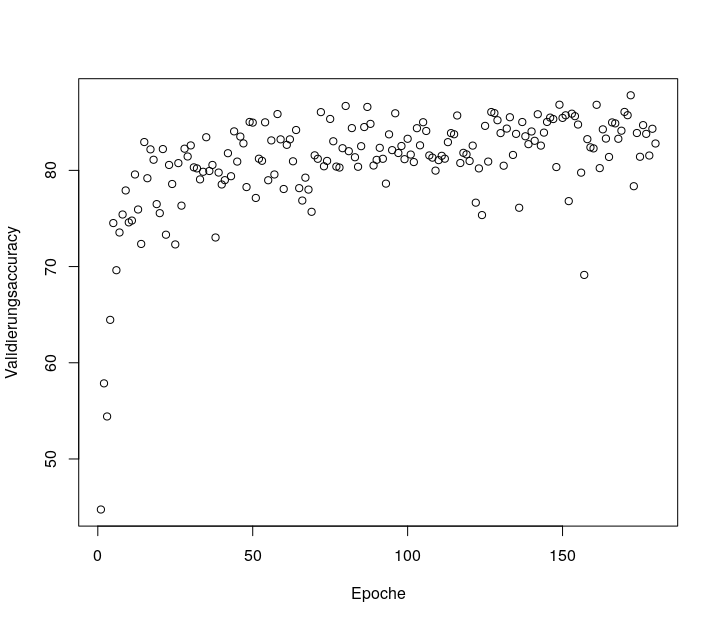
\includegraphics[width=1\linewidth]{KapitelPartB/Images/BaseAcc1.png}
      \caption{Accuracy Baseline Netz ohne Anpassung der Lernrate}
      \label{abb:baseAcc1}
      \end{minipage}
   \begin{minipage}[c]{.45\linewidth} % [b] => Ausrichtung an \caption
      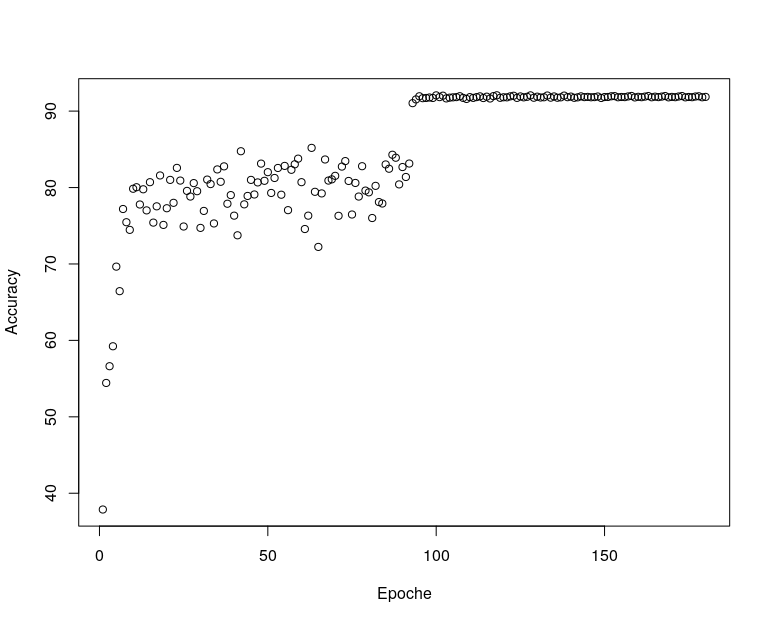
\includegraphics[width=1\linewidth]{KapitelPartB/Images/BaseAcc2.png}
      \caption{Übergangsblock}
      \label{abb:baseAcc2}
   \end{minipage}
   \label{abb:blocks}
\end{figure}

Die Durchschnittswerte und Standardabweichungen für die zehn Baseline Experimente sind in Tabelle \ref{tab:baseline} aufgelsitet. Die Durchschnittswerte liegen sehr nah beeinander, der Unterschied zwischen dem grössten und dem kleinsten liegt bei xx,xx, womit sich eine Abweichung von xx,xx \% ergibt. Durch die maximale Standardabweichung von xx,xx haben auch alle übrigen Werte eine maximale durchschnittliche Abweichung von xx,xx. Damit ergeben sich zwischen den zehn Experimenten keine signifikante Unterschiede. Es wird daher mit Experiment 6 eines der Experimente mit Anpassung der Lernrate ausgesucht um für die folgenden Experimente/ Kapitel als Vergleich zu dienen.
\begin{table}[h]
\begin{tabular}{|l|l|l|l|l|l|l|l|l|l|l|} \hline
           & \multicolumn{5}{c|}{Experimente ohne Anpassung}&\multicolumn{5}{c|}{Experimente mit Anpassung} \\
           &\multicolumn{5}{c|}{der Lernrate} &\multicolumn{5}{c|}{der Lernrate}\\
           & 1       & 2      & 3      & 4       & 5       & 6   & 7 & 8      & 9      & 10 \\ \hline 
$\mu$      & 137,57  & 137,98 & 138,43 & 139,14  & 138,73  &     &   & 145,83 & 145,81 & 145.19  \\ \hline
$\sigma$   & 15,10   & 9,72   & 8,51   & 10,67   & 10,77   &     &   & 12.12  & 11.55  & 12.40  \\ \hline
\end{tabular}
\caption{Tabelle für Durchschnittswerte und Standardabweichungen der Experimente}
\label{tab:baseline}
\end{table}

\section{Konzept}\label{sec:konzept}




In diesem Kapitel werden verschiedenen Methoden, die in Kapitel 2 Vorgestellt wurden, auf einer Grafikkarte ausgeführt, evaluiert und die Ergebnisse verglichen. In Kapitel \ref{sec:setup} werden zunächst das experimentelle Setup vorgestellt. In Kapitel \ref{sec:ptexperimente} wird das Beschneiden des Netzes zunächst so getestet, wie es in der vorgefertigten Implementierung hinterlegt ist \cite{ptImpl}. In Kapitel \ref{pt:new} wird dann untersucht wie sich das Beschneiden des Netzes mit zusätzlicher Anpassung der Batchgrösse verhält.

Die beiden Operatorn, die das Netz tiefer beziehungsweise breiter machen werden in Kapitel \ref{sec:net2netexperimente} durch Experimente evaluiert. In Kapitel \ref{sec:ptpnet2net} werden dann die Operatoren für ein breiteres Netz beziehungsweise ein tieferes Netz mit der Technik des Beschneidens der Netze kombiniert, um ein automatisches Suchen einer besseren Architektur zu ermöglichen. Diese Verbindung wird dann mit dem Schnellen Ressourcen beschränktem Strukturlernen tiefer Netze verglichen. Das Strukturlernen wird dafür zunächst in Kapitel \ref{sec:morphexperimente} evaluiert. Der Vergleich der Ergebnisse wird dann in Kapitel \ref{sec:vergleich} gemacht.


Zuletzt werden noch additive Verfahren vorgetellt, welche die Trainingszeit zusätzlich minimieren können.
Eine dieser Verfahren, welches in Kapitel \ref{sec:zahlen} evaluiert wird, spart Zeit durch die Verwendung von gemischt präzisen Zahlenformaten.

Ein weiteres additives Verfahren in Kapitel \ref{sec:lars} überprüft in wiefern mit Hilfe einer adaptiven Anpassung der Lernrate die Batchgröße sinvoll so angepasst werden kann, dass die ganze GPU genutzt werden kann.


\color{black}
